\documentclass[twoside]{book}

% Packages required by doxygen
\usepackage{calc}
\usepackage{doxygen}
\usepackage{graphicx}
\usepackage[utf8]{inputenc}
\usepackage{makeidx}
\usepackage{multicol}
\usepackage{multirow}
\usepackage{fixltx2e}
\PassOptionsToPackage{warn}{textcomp}
\usepackage{textcomp}
\usepackage[nointegrals]{wasysym}
\usepackage[table]{xcolor}

% NLS support packages
\usepackage[T2A]{fontenc}
\usepackage[russian]{babel}

% Font selection
\usepackage[T1]{fontenc}
\usepackage{mathptmx}
\usepackage[scaled=.90]{helvet}
\usepackage{courier}
\usepackage{amssymb}
\usepackage{sectsty}
\renewcommand{\familydefault}{\sfdefault}
\allsectionsfont{%
  \fontseries{bc}\selectfont%
  \color{darkgray}%
}
\renewcommand{\DoxyLabelFont}{%
  \fontseries{bc}\selectfont%
  \color{darkgray}%
}
\newcommand{\+}{\discretionary{\mbox{\scriptsize$\hookleftarrow$}}{}{}}

% Page & text layout
\usepackage{geometry}
\geometry{%
  a4paper,%
  top=2.5cm,%
  bottom=2.5cm,%
  left=2.5cm,%
  right=2.5cm%
}
\tolerance=750
\hfuzz=15pt
\hbadness=750
\setlength{\emergencystretch}{15pt}
\setlength{\parindent}{0cm}
\setlength{\parskip}{0.2cm}
\makeatletter
\renewcommand{\paragraph}{%
  \@startsection{paragraph}{4}{0ex}{-1.0ex}{1.0ex}{%
    \normalfont\normalsize\bfseries\SS@parafont%
  }%
}
\renewcommand{\subparagraph}{%
  \@startsection{subparagraph}{5}{0ex}{-1.0ex}{1.0ex}{%
    \normalfont\normalsize\bfseries\SS@subparafont%
  }%
}
\makeatother

% Headers & footers
\usepackage{fancyhdr}
\pagestyle{fancyplain}
\fancyhead[LE]{\fancyplain{}{\bfseries\thepage}}
\fancyhead[CE]{\fancyplain{}{}}
\fancyhead[RE]{\fancyplain{}{\bfseries\leftmark}}
\fancyhead[LO]{\fancyplain{}{\bfseries\rightmark}}
\fancyhead[CO]{\fancyplain{}{}}
\fancyhead[RO]{\fancyplain{}{\bfseries\thepage}}
\fancyfoot[LE]{\fancyplain{}{}}
\fancyfoot[CE]{\fancyplain{}{}}
\fancyfoot[RE]{\fancyplain{}{\bfseries\scriptsize Документация по Advert\+Data. Последние изменения\+: Ср 18 Июн 2014 12\+:04\+:59. Создано системой Doxygen }}
\fancyfoot[LO]{\fancyplain{}{\bfseries\scriptsize Документация по Advert\+Data. Последние изменения\+: Ср 18 Июн 2014 12\+:04\+:59. Создано системой Doxygen }}
\fancyfoot[CO]{\fancyplain{}{}}
\fancyfoot[RO]{\fancyplain{}{}}
\renewcommand{\footrulewidth}{0.4pt}
\renewcommand{\chaptermark}[1]{%
  \markboth{#1}{}%
}
\renewcommand{\sectionmark}[1]{%
  \markright{\thesection\ #1}%
}

% Indices & bibliography
\usepackage{natbib}
\usepackage[titles]{tocloft}
\setcounter{tocdepth}{3}
\setcounter{secnumdepth}{5}
\makeindex

% Hyperlinks (required, but should be loaded last)
\usepackage{ifpdf}
\ifpdf
  \usepackage[pdftex,pagebackref=true]{hyperref}
\else
  \usepackage[ps2pdf,pagebackref=true]{hyperref}
\fi
\hypersetup{%
  colorlinks=true,%
  linkcolor=blue,%
  citecolor=blue,%
  unicode%
}

% Custom commands
\newcommand{\clearemptydoublepage}{%
  \newpage{\pagestyle{empty}\cleardoublepage}%
}


%===== C O N T E N T S =====

\begin{document}

% Titlepage & ToC
\hypersetup{pageanchor=false,
             bookmarks=true,
             bookmarksnumbered=true,
             pdfencoding=unicode
            }
\pagenumbering{roman}
\begin{titlepage}
\vspace*{7cm}
\begin{center}%
{\Large Advert\+Data }\\
\vspace*{1cm}
{\large Создано системой Doxygen 1.8.7}\\
\vspace*{0.5cm}
{\small Ср 18 Июн 2014 12:04:59}\\
\end{center}
\end{titlepage}
\clearemptydoublepage
\tableofcontents
\clearemptydoublepage
\pagenumbering{arabic}
\hypersetup{pageanchor=true}

%--- Begin generated contents ---
\chapter{Алфавитный указатель пространств имен}
\section{Пакеты}
Полный список документированных пакетов.\begin{DoxyCompactList}
\item\contentsline{section}{\hyperlink{namespace_advert_data}{Advert\+Data} }{\pageref{namespace_advert_data}}{}
\item\contentsline{section}{\hyperlink{namespace_advert_data_1_1_editor}{Advert\+Data.\+Editor} }{\pageref{namespace_advert_data_1_1_editor}}{}
\item\contentsline{section}{\hyperlink{namespace_advert_data_1_1_editor_1_1_properties}{Advert\+Data.\+Editor.\+Properties} }{\pageref{namespace_advert_data_1_1_editor_1_1_properties}}{}
\item\contentsline{section}{\hyperlink{namespace_advert_data_1_1_forms}{Advert\+Data.\+Forms} }{\pageref{namespace_advert_data_1_1_forms}}{}
\end{DoxyCompactList}

\chapter{Иерархический список классов}
\section{Иерархия классов}
Иерархия классов.\begin{DoxyCompactList}
\item \contentsline{section}{Advert\+Data.\+Database}{\pageref{class_advert_data_1_1_database}}{}
\item Form\begin{DoxyCompactList}
\item \contentsline{section}{Advert\+Data.\+Forms.\+Advert\+Data\+Form}{\pageref{class_advert_data_1_1_forms_1_1_advert_data_form}}{}
\end{DoxyCompactList}
\item \contentsline{section}{Advert\+Data.\+Record}{\pageref{class_advert_data_1_1_record}}{}
\item \contentsline{section}{Advert\+Data.\+Settings}{\pageref{class_advert_data_1_1_settings}}{}
\end{DoxyCompactList}

\chapter{Алфавитный указатель классов}
\section{Классы}
Классы с их кратким описанием.\begin{DoxyCompactList}
\item\contentsline{section}{\hyperlink{class_advert_data_1_1_forms_1_1_advert_data_form}{Advert\+Data.\+Forms.\+Advert\+Data\+Form} \\*Форма для отображения отчёта Пример использования Application.\+Run(new Advert\+Data\+Form(new Database())); }{\pageref{class_advert_data_1_1_forms_1_1_advert_data_form}}{}
\item\contentsline{section}{\hyperlink{class_advert_data_1_1_database}{Advert\+Data.\+Database} \\*Класс для работы с базой данных }{\pageref{class_advert_data_1_1_database}}{}
\item\contentsline{section}{\hyperlink{class_advert_data_1_1_record}{Advert\+Data.\+Record} }{\pageref{class_advert_data_1_1_record}}{}
\item\contentsline{section}{\hyperlink{class_advert_data_1_1_settings}{Advert\+Data.\+Settings} \\*Класс для хранения настроечных параметров модуля }{\pageref{class_advert_data_1_1_settings}}{}
\end{DoxyCompactList}

\chapter{Пространства имен}
\hypertarget{namespace_advert_data}{\section{Пакет Advert\+Data}
\label{namespace_advert_data}\index{Advert\+Data@{Advert\+Data}}
}
\subsection*{Пространства имен}
\begin{DoxyCompactItemize}
\item 
package \hyperlink{namespace_advert_data_1_1_editor}{Editor}
\item 
package \hyperlink{namespace_advert_data_1_1_forms}{Forms}
\end{DoxyCompactItemize}
\subsection*{Классы}
\begin{DoxyCompactItemize}
\item 
class \hyperlink{class_advert_data_1_1_database}{Database}
\begin{DoxyCompactList}\small\item\em Класс для работы с базой данных \end{DoxyCompactList}\item 
class {\bfseries Db\+Type\+Attribute}
\item 
class {\bfseries Key\+Attribute}
\item 
class \hyperlink{class_advert_data_1_1_record}{Record}
\item 
class \hyperlink{class_advert_data_1_1_settings}{Settings}
\begin{DoxyCompactList}\small\item\em Класс для хранения настроечных параметров модуля \end{DoxyCompactList}\item 
class {\bfseries Value\+Attribute}
\end{DoxyCompactItemize}

\hypertarget{namespace_advert_data_1_1_editor}{\section{Пакет Advert\+Data.\+Editor}
\label{namespace_advert_data_1_1_editor}\index{Advert\+Data.\+Editor@{Advert\+Data.\+Editor}}
}
\subsection*{Пространства имен}
\begin{DoxyCompactItemize}
\item 
package \hyperlink{namespace_advert_data_1_1_editor_1_1_properties}{Properties}
\end{DoxyCompactItemize}
\subsection*{Классы}
\begin{DoxyCompactItemize}
\item 
class {\bfseries Program}
\end{DoxyCompactItemize}

\hypertarget{namespace_advert_data_1_1_editor_1_1_properties}{\section{Пакет Advert\+Data.\+Editor.\+Properties}
\label{namespace_advert_data_1_1_editor_1_1_properties}\index{Advert\+Data.\+Editor.\+Properties@{Advert\+Data.\+Editor.\+Properties}}
}
\subsection*{Классы}
\begin{DoxyCompactItemize}
\item 
class {\bfseries Resources}
\begin{DoxyCompactList}\small\item\em Класс ресурсов со строгим типом для поиска локализованных строк и пр. \end{DoxyCompactList}\item 
class {\bfseries Settings}
\end{DoxyCompactItemize}

\hypertarget{namespace_advert_data_1_1_forms}{\section{Пакет Advert\+Data.\+Forms}
\label{namespace_advert_data_1_1_forms}\index{Advert\+Data.\+Forms@{Advert\+Data.\+Forms}}
}
\subsection*{Классы}
\begin{DoxyCompactItemize}
\item 
class \hyperlink{class_advert_data_1_1_forms_1_1_advert_data_form}{Advert\+Data\+Form}
\begin{DoxyCompactList}\small\item\em Форма для отображения отчёта Пример использования Application.\+Run(new Advert\+Data\+Form(new Database())); \end{DoxyCompactList}\end{DoxyCompactItemize}

\chapter{Классы}
\hypertarget{class_advert_data_1_1_forms_1_1_advert_data_form}{\section{Класс Advert\+Data.\+Forms.\+Advert\+Data\+Form}
\label{class_advert_data_1_1_forms_1_1_advert_data_form}\index{Advert\+Data.\+Forms.\+Advert\+Data\+Form@{Advert\+Data.\+Forms.\+Advert\+Data\+Form}}
}


Форма для отображения отчёта Пример использования Application.\+Run(new Advert\+Data\+Form(new Database()));  


Граф наследования\+:Advert\+Data.\+Forms.\+Advert\+Data\+Form\+:\begin{figure}[H]
\begin{center}
\leavevmode
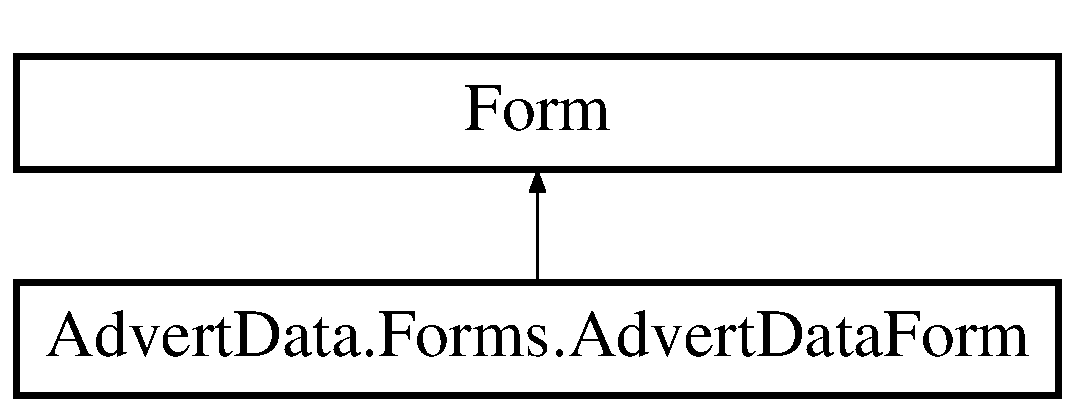
\includegraphics[height=2.000000cm]{class_advert_data_1_1_forms_1_1_advert_data_form}
\end{center}
\end{figure}
\subsection*{Открытые члены}
\begin{DoxyCompactItemize}
\item 
\hyperlink{class_advert_data_1_1_forms_1_1_advert_data_form_ade74bad239228075b06f23f00652bb55}{Advert\+Data\+Form} (\hyperlink{class_advert_data_1_1_database}{Database} database)
\begin{DoxyCompactList}\small\item\em Форма для отображения отчёта Пример использования Application.\+Run(new Advert\+Data\+Form(new Database())); \end{DoxyCompactList}\end{DoxyCompactItemize}
\subsection*{Защищенные члены}
\begin{DoxyCompactItemize}
\item 
override void \hyperlink{class_advert_data_1_1_forms_1_1_advert_data_form_a657f930ffab20a51d5f5949e7e1c0922}{Dispose} (bool disposing)
\begin{DoxyCompactList}\small\item\em Clean up any resources being used. \end{DoxyCompactList}\end{DoxyCompactItemize}
\subsection*{Свойства}
\begin{DoxyCompactItemize}
\item 
bool \hyperlink{class_advert_data_1_1_forms_1_1_advert_data_form_a0a8f6aa3373c003f390580a4b91dfe64}{Report}\hspace{0.3cm}{\ttfamily  \mbox{[}get, set\mbox{]}}
\begin{DoxyCompactList}\small\item\em флаг «Вести отчет» устанавливает значение в True или False переменной Report отдельной таблицы проекта \hyperlink{class_advert_data_1_1_settings}{Settings} и на данный отчет или методы никак не влияет. Данный фильтр нужен для других механизмов проекта, но управляется из этого интерфейса. D\+L\+L должна содержать методы управления флагом, а так же метод определения состояния флага. Соединение с базой данных должно быть установлено перед использованием свойства. \end{DoxyCompactList}\end{DoxyCompactItemize}


\subsection{Подробное описание}
Форма для отображения отчёта Пример использования Application.\+Run(new Advert\+Data\+Form(new Database())); 



\subsection{Конструктор(ы)}
\hypertarget{class_advert_data_1_1_forms_1_1_advert_data_form_ade74bad239228075b06f23f00652bb55}{\index{Advert\+Data\+::\+Forms\+::\+Advert\+Data\+Form@{Advert\+Data\+::\+Forms\+::\+Advert\+Data\+Form}!Advert\+Data\+Form@{Advert\+Data\+Form}}
\index{Advert\+Data\+Form@{Advert\+Data\+Form}!Advert\+Data\+::\+Forms\+::\+Advert\+Data\+Form@{Advert\+Data\+::\+Forms\+::\+Advert\+Data\+Form}}
\subsubsection[{Advert\+Data\+Form}]{\setlength{\rightskip}{0pt plus 5cm}Advert\+Data.\+Forms.\+Advert\+Data\+Form.\+Advert\+Data\+Form (
\begin{DoxyParamCaption}
\item[{{\bf Database}}]{database}
\end{DoxyParamCaption}
)}}\label{class_advert_data_1_1_forms_1_1_advert_data_form_ade74bad239228075b06f23f00652bb55}


Форма для отображения отчёта Пример использования Application.\+Run(new Advert\+Data\+Form(new Database())); 


\begin{DoxyParams}{Аргументы}
{\em database} & \\
\hline
\end{DoxyParams}


\subsection{Методы}
\hypertarget{class_advert_data_1_1_forms_1_1_advert_data_form_a657f930ffab20a51d5f5949e7e1c0922}{\index{Advert\+Data\+::\+Forms\+::\+Advert\+Data\+Form@{Advert\+Data\+::\+Forms\+::\+Advert\+Data\+Form}!Dispose@{Dispose}}
\index{Dispose@{Dispose}!Advert\+Data\+::\+Forms\+::\+Advert\+Data\+Form@{Advert\+Data\+::\+Forms\+::\+Advert\+Data\+Form}}
\subsubsection[{Dispose}]{\setlength{\rightskip}{0pt plus 5cm}override void Advert\+Data.\+Forms.\+Advert\+Data\+Form.\+Dispose (
\begin{DoxyParamCaption}
\item[{bool}]{disposing}
\end{DoxyParamCaption}
)\hspace{0.3cm}{\ttfamily [protected]}}}\label{class_advert_data_1_1_forms_1_1_advert_data_form_a657f930ffab20a51d5f5949e7e1c0922}


Clean up any resources being used. 


\begin{DoxyParams}{Аргументы}
{\em disposing} & true if managed resources should be disposed; otherwise, false.\\
\hline
\end{DoxyParams}


\subsection{Полный список свойств}
\hypertarget{class_advert_data_1_1_forms_1_1_advert_data_form_a0a8f6aa3373c003f390580a4b91dfe64}{\index{Advert\+Data\+::\+Forms\+::\+Advert\+Data\+Form@{Advert\+Data\+::\+Forms\+::\+Advert\+Data\+Form}!Report@{Report}}
\index{Report@{Report}!Advert\+Data\+::\+Forms\+::\+Advert\+Data\+Form@{Advert\+Data\+::\+Forms\+::\+Advert\+Data\+Form}}
\subsubsection[{Report}]{\setlength{\rightskip}{0pt plus 5cm}bool Advert\+Data.\+Forms.\+Advert\+Data\+Form.\+Report\hspace{0.3cm}{\ttfamily [get]}, {\ttfamily [set]}}}\label{class_advert_data_1_1_forms_1_1_advert_data_form_a0a8f6aa3373c003f390580a4b91dfe64}


флаг «Вести отчет» устанавливает значение в True или False переменной Report отдельной таблицы проекта \hyperlink{class_advert_data_1_1_settings}{Settings} и на данный отчет или методы никак не влияет. Данный фильтр нужен для других механизмов проекта, но управляется из этого интерфейса. D\+L\+L должна содержать методы управления флагом, а так же метод определения состояния флага. Соединение с базой данных должно быть установлено перед использованием свойства. 



Объявления и описания членов классов находятся в файлах\+:\begin{DoxyCompactItemize}
\item 
Advert\+Data/\+Forms/Advert\+Data\+Form.\+cs\item 
Advert\+Data/\+Forms/Advert\+Data\+Form.\+Designer.\+cs\end{DoxyCompactItemize}

\hypertarget{class_advert_data_1_1_database}{\section{Класс Advert\+Data.\+Database}
\label{class_advert_data_1_1_database}\index{Advert\+Data.\+Database@{Advert\+Data.\+Database}}
}


Класс для работы с базой данных  


\subsection*{Открытые члены}
\begin{DoxyCompactItemize}
\item 
void \hyperlink{class_advert_data_1_1_database_a411697c67e1f4b3b8669850e33f61cdc}{Connect} ()
\begin{DoxyCompactList}\small\item\em Метод инициализации к базе данных \end{DoxyCompactList}\item 
void \hyperlink{class_advert_data_1_1_database_a17d29da3fd0335e2bbb53ba149e71c3b}{Disconnect} ()
\begin{DoxyCompactList}\small\item\em Метод отключения от базы данных \end{DoxyCompactList}\item 
void \hyperlink{class_advert_data_1_1_database_a91140db43510a4eb52de88bf5ef34dc9}{Clear\+All\+Report} ()
\begin{DoxyCompactList}\small\item\em Очищает всю БД отчета. \end{DoxyCompactList}\item 
void \hyperlink{class_advert_data_1_1_database_a78c39f11605ed7527d1858e84e0b2334}{Remove\+Start\+Time} (string date\+Time1=null, string date\+Time2=null)
\begin{DoxyCompactList}\small\item\em Метод удаляет Start\+Time и все связи от этого Start\+Time к остальным полям с каскадным удалением этих полей. Т.\+е. удаление этих полей, если на них больше никто не ссылается. Все исходные данные хранятся в одной таблице, поэтому список Start\+Time-\/ов является всего лишь выборой уникальных значений Start\+Time из этой таблицы \end{DoxyCompactList}\item 
void \hyperlink{class_advert_data_1_1_database_a5e68ba2819a0aa1da8a266fb194c3f31}{Add\+Start\+Time} (string date\+Time)
\begin{DoxyCompactList}\small\item\em Создает новую запись Start\+Time. Данный метод является заглушкой -\/ то есть не выполняет никаких действий. Все исходные данные хранятся в одной таблице, поэтому список Start\+Time-\/ов является всего лишь выборой уникальных значений Start\+Time из этой таблицы \end{DoxyCompactList}\item 
bool \hyperlink{class_advert_data_1_1_database_a6d68c71acccd791dbabc11b69af15656}{Exists} (string date\+Time)
\begin{DoxyCompactList}\small\item\em Проверка существования записей с указанной датой \end{DoxyCompactList}\item 
string \hyperlink{class_advert_data_1_1_database_acd02f2b52c12782c264db0041e9f6ffb}{Get\+Setting} (string name)
\begin{DoxyCompactList}\small\item\em Получение значения настроечного параметра \end{DoxyCompactList}\item 
\hypertarget{class_advert_data_1_1_database_a7fd09fc8bf0c77fb716156ce482942cd}{I\+Enumerable$<$ string $>$ {\bfseries Get\+Start\+Dates} ()}\label{class_advert_data_1_1_database_a7fd09fc8bf0c77fb716156ce482942cd}

\item 
bool \hyperlink{class_advert_data_1_1_database_a1035e18ac4389569bc236236f850d9c3}{Set\+Data} (string start\+Time, string key, string dll, string resource, string url, string user, string result, string ad=null)
\begin{DoxyCompactList}\small\item\em Метод находит запись со значением Start\+Time и к ней добавляет остальные данные. В поле Time прописывает текущее время записи. Возвращает False если Start\+Time не найдена. \end{DoxyCompactList}\item 
I\+Enumerable$<$ \hyperlink{class_advert_data_1_1_record}{Record} $>$ \hyperlink{class_advert_data_1_1_database_a31db3b29faa658c6b559c8a02d2d683d}{Get\+Data} (string date\+Time1, string date\+Time2)
\begin{DoxyCompactList}\small\item\em Получение списка записей, находящихся в указанном диапазоне дат (включительно) фильтр «показать отчет с … по…» если не задан, то таблица отображает все данные. Если задан одно значение «показать отчет с…», то таблица отображает данные с указанного периода до конца значений; Если задан одно значение «показать отчет по…», то таблица отображает данные с самого начала до указанного значения; Если заданны оба значения, то таблица отображает данные входящие в этот период; Данный фильтр ведется только по полю Start\+Time, т.\+е отображаются данные Start\+Time попавшие в фильтр и все привязанные к нему данные даже если Time привязанных записей выпадает за пределы фильтра. \end{DoxyCompactList}\item 
void \hyperlink{class_advert_data_1_1_database_a1f0ff57f6d508514c5aaf02dca134de3}{Set\+Setting} (string name, string value)
\begin{DoxyCompactList}\small\item\em Установка значения настроечного параметра \end{DoxyCompactList}\end{DoxyCompactItemize}
\subsection*{Свойства}
\begin{DoxyCompactItemize}
\item 
bool \hyperlink{class_advert_data_1_1_database_a792a2c162be5a913573b560fc0d9cb3f}{Report}\hspace{0.3cm}{\ttfamily  \mbox{[}get, set\mbox{]}}
\begin{DoxyCompactList}\small\item\em флаг «Вести отчет» устанавливает значение в True или False переменной Report отдельной таблицы проекта и на данный отчет или методы никак не влияет. Данный фильтр нужен для других механизмов проекта, но управляется из этого интерфейса. D\+L\+L должна содержать методы управления флагом, а так же метод определения состояния флага. \end{DoxyCompactList}\item 
object \hyperlink{class_advert_data_1_1_database_a4ff9641ffa4a8b7431228d126703928c}{Semaphore}\hspace{0.3cm}{\ttfamily  \mbox{[}get, set\mbox{]}}
\begin{DoxyCompactList}\small\item\em Семафор для блокирования одновременного доступа к классу из параллельных процессов Использование lock(database.\+Semaphore) \{ ... \} \end{DoxyCompactList}\end{DoxyCompactItemize}


\subsection{Подробное описание}
Класс для работы с базой данных 



\subsection{Методы}
\hypertarget{class_advert_data_1_1_database_a5e68ba2819a0aa1da8a266fb194c3f31}{\index{Advert\+Data\+::\+Database@{Advert\+Data\+::\+Database}!Add\+Start\+Time@{Add\+Start\+Time}}
\index{Add\+Start\+Time@{Add\+Start\+Time}!Advert\+Data\+::\+Database@{Advert\+Data\+::\+Database}}
\subsubsection[{Add\+Start\+Time}]{\setlength{\rightskip}{0pt plus 5cm}void Advert\+Data.\+Database.\+Add\+Start\+Time (
\begin{DoxyParamCaption}
\item[{string}]{date\+Time}
\end{DoxyParamCaption}
)}}\label{class_advert_data_1_1_database_a5e68ba2819a0aa1da8a266fb194c3f31}


Создает новую запись Start\+Time. Данный метод является заглушкой -\/ то есть не выполняет никаких действий. Все исходные данные хранятся в одной таблице, поэтому список Start\+Time-\/ов является всего лишь выборой уникальных значений Start\+Time из этой таблицы 


\begin{DoxyParams}{Аргументы}
{\em date\+Time} & Дата и время с учетом миллисекунд\\
\hline
\end{DoxyParams}
\hypertarget{class_advert_data_1_1_database_a91140db43510a4eb52de88bf5ef34dc9}{\index{Advert\+Data\+::\+Database@{Advert\+Data\+::\+Database}!Clear\+All\+Report@{Clear\+All\+Report}}
\index{Clear\+All\+Report@{Clear\+All\+Report}!Advert\+Data\+::\+Database@{Advert\+Data\+::\+Database}}
\subsubsection[{Clear\+All\+Report}]{\setlength{\rightskip}{0pt plus 5cm}void Advert\+Data.\+Database.\+Clear\+All\+Report (
\begin{DoxyParamCaption}
{}
\end{DoxyParamCaption}
)}}\label{class_advert_data_1_1_database_a91140db43510a4eb52de88bf5ef34dc9}


Очищает всю БД отчета. 

\hypertarget{class_advert_data_1_1_database_a411697c67e1f4b3b8669850e33f61cdc}{\index{Advert\+Data\+::\+Database@{Advert\+Data\+::\+Database}!Connect@{Connect}}
\index{Connect@{Connect}!Advert\+Data\+::\+Database@{Advert\+Data\+::\+Database}}
\subsubsection[{Connect}]{\setlength{\rightskip}{0pt plus 5cm}void Advert\+Data.\+Database.\+Connect (
\begin{DoxyParamCaption}
{}
\end{DoxyParamCaption}
)}}\label{class_advert_data_1_1_database_a411697c67e1f4b3b8669850e33f61cdc}


Метод инициализации к базе данных 

\hypertarget{class_advert_data_1_1_database_a17d29da3fd0335e2bbb53ba149e71c3b}{\index{Advert\+Data\+::\+Database@{Advert\+Data\+::\+Database}!Disconnect@{Disconnect}}
\index{Disconnect@{Disconnect}!Advert\+Data\+::\+Database@{Advert\+Data\+::\+Database}}
\subsubsection[{Disconnect}]{\setlength{\rightskip}{0pt plus 5cm}void Advert\+Data.\+Database.\+Disconnect (
\begin{DoxyParamCaption}
{}
\end{DoxyParamCaption}
)}}\label{class_advert_data_1_1_database_a17d29da3fd0335e2bbb53ba149e71c3b}


Метод отключения от базы данных 

\hypertarget{class_advert_data_1_1_database_a6d68c71acccd791dbabc11b69af15656}{\index{Advert\+Data\+::\+Database@{Advert\+Data\+::\+Database}!Exists@{Exists}}
\index{Exists@{Exists}!Advert\+Data\+::\+Database@{Advert\+Data\+::\+Database}}
\subsubsection[{Exists}]{\setlength{\rightskip}{0pt plus 5cm}bool Advert\+Data.\+Database.\+Exists (
\begin{DoxyParamCaption}
\item[{string}]{date\+Time}
\end{DoxyParamCaption}
)}}\label{class_advert_data_1_1_database_a6d68c71acccd791dbabc11b69af15656}


Проверка существования записей с указанной датой 


\begin{DoxyParams}{Аргументы}
{\em date\+Time} & Дата и время с учетом миллисекунд\\
\hline
\end{DoxyParams}
\begin{DoxyReturn}{Возвращает}
Признак существования записей с указанной датой
\end{DoxyReturn}
\hypertarget{class_advert_data_1_1_database_a31db3b29faa658c6b559c8a02d2d683d}{\index{Advert\+Data\+::\+Database@{Advert\+Data\+::\+Database}!Get\+Data@{Get\+Data}}
\index{Get\+Data@{Get\+Data}!Advert\+Data\+::\+Database@{Advert\+Data\+::\+Database}}
\subsubsection[{Get\+Data}]{\setlength{\rightskip}{0pt plus 5cm}I\+Enumerable$<${\bf Record}$>$ Advert\+Data.\+Database.\+Get\+Data (
\begin{DoxyParamCaption}
\item[{string}]{date\+Time1, }
\item[{string}]{date\+Time2}
\end{DoxyParamCaption}
)}}\label{class_advert_data_1_1_database_a31db3b29faa658c6b559c8a02d2d683d}


Получение списка записей, находящихся в указанном диапазоне дат (включительно) фильтр «показать отчет с … по…» если не задан, то таблица отображает все данные. Если задан одно значение «показать отчет с…», то таблица отображает данные с указанного периода до конца значений; Если задан одно значение «показать отчет по…», то таблица отображает данные с самого начала до указанного значения; Если заданны оба значения, то таблица отображает данные входящие в этот период; Данный фильтр ведется только по полю Start\+Time, т.\+е отображаются данные Start\+Time попавшие в фильтр и все привязанные к нему данные даже если Time привязанных записей выпадает за пределы фильтра. 


\begin{DoxyParams}{Аргументы}
{\em date\+Time1} & Минимальная дата и время с учетом миллисекунд. Допустимо значение null.\\
\hline
{\em date\+Time2} & Максимальная дата и время с учетом миллисекунд. Допустимо значение null.\\
\hline
\end{DoxyParams}
\begin{DoxyReturn}{Возвращает}
Список записей
\end{DoxyReturn}
\hypertarget{class_advert_data_1_1_database_acd02f2b52c12782c264db0041e9f6ffb}{\index{Advert\+Data\+::\+Database@{Advert\+Data\+::\+Database}!Get\+Setting@{Get\+Setting}}
\index{Get\+Setting@{Get\+Setting}!Advert\+Data\+::\+Database@{Advert\+Data\+::\+Database}}
\subsubsection[{Get\+Setting}]{\setlength{\rightskip}{0pt plus 5cm}string Advert\+Data.\+Database.\+Get\+Setting (
\begin{DoxyParamCaption}
\item[{string}]{name}
\end{DoxyParamCaption}
)}}\label{class_advert_data_1_1_database_acd02f2b52c12782c264db0041e9f6ffb}


Получение значения настроечного параметра 


\begin{DoxyParams}{Аргументы}
{\em name} & Имя настроечного параметра\\
\hline
\end{DoxyParams}
\begin{DoxyReturn}{Возвращает}
Значение настроечного параметра
\end{DoxyReturn}
\hypertarget{class_advert_data_1_1_database_a78c39f11605ed7527d1858e84e0b2334}{\index{Advert\+Data\+::\+Database@{Advert\+Data\+::\+Database}!Remove\+Start\+Time@{Remove\+Start\+Time}}
\index{Remove\+Start\+Time@{Remove\+Start\+Time}!Advert\+Data\+::\+Database@{Advert\+Data\+::\+Database}}
\subsubsection[{Remove\+Start\+Time}]{\setlength{\rightskip}{0pt plus 5cm}void Advert\+Data.\+Database.\+Remove\+Start\+Time (
\begin{DoxyParamCaption}
\item[{string}]{date\+Time1 = {\ttfamily null}, }
\item[{string}]{date\+Time2 = {\ttfamily null}}
\end{DoxyParamCaption}
)}}\label{class_advert_data_1_1_database_a78c39f11605ed7527d1858e84e0b2334}


Метод удаляет Start\+Time и все связи от этого Start\+Time к остальным полям с каскадным удалением этих полей. Т.\+е. удаление этих полей, если на них больше никто не ссылается. Все исходные данные хранятся в одной таблице, поэтому список Start\+Time-\/ов является всего лишь выборой уникальных значений Start\+Time из этой таблицы 


\begin{DoxyParams}{Аргументы}
{\em date\+Time1} & Минимальная дата и время с учетом миллисекунд. Допустимо значение null.\\
\hline
{\em date\+Time2} & Максимальная дата и время с учетом миллисекунд. Допустимо значение null.\\
\hline
\end{DoxyParams}
\hypertarget{class_advert_data_1_1_database_a1035e18ac4389569bc236236f850d9c3}{\index{Advert\+Data\+::\+Database@{Advert\+Data\+::\+Database}!Set\+Data@{Set\+Data}}
\index{Set\+Data@{Set\+Data}!Advert\+Data\+::\+Database@{Advert\+Data\+::\+Database}}
\subsubsection[{Set\+Data}]{\setlength{\rightskip}{0pt plus 5cm}bool Advert\+Data.\+Database.\+Set\+Data (
\begin{DoxyParamCaption}
\item[{string}]{start\+Time, }
\item[{string}]{key, }
\item[{string}]{dll, }
\item[{string}]{resource, }
\item[{string}]{url, }
\item[{string}]{user, }
\item[{string}]{result, }
\item[{string}]{ad = {\ttfamily null}}
\end{DoxyParamCaption}
)}}\label{class_advert_data_1_1_database_a1035e18ac4389569bc236236f850d9c3}


Метод находит запись со значением Start\+Time и к ней добавляет остальные данные. В поле Time прописывает текущее время записи. Возвращает False если Start\+Time не найдена. 


\begin{DoxyParams}{Аргументы}
{\em start\+Time} & Время начала выполнения\\
\hline
{\em key} & \\
\hline
{\em dll} & \\
\hline
{\em resource} & \\
\hline
{\em url} & \\
\hline
{\em user} & \\
\hline
{\em result} & \\
\hline
{\em ad} & \\
\hline
\end{DoxyParams}
\begin{DoxyReturn}{Возвращает}
Признак существования записей с указанной датой
\end{DoxyReturn}
\hypertarget{class_advert_data_1_1_database_a1f0ff57f6d508514c5aaf02dca134de3}{\index{Advert\+Data\+::\+Database@{Advert\+Data\+::\+Database}!Set\+Setting@{Set\+Setting}}
\index{Set\+Setting@{Set\+Setting}!Advert\+Data\+::\+Database@{Advert\+Data\+::\+Database}}
\subsubsection[{Set\+Setting}]{\setlength{\rightskip}{0pt plus 5cm}void Advert\+Data.\+Database.\+Set\+Setting (
\begin{DoxyParamCaption}
\item[{string}]{name, }
\item[{string}]{value}
\end{DoxyParamCaption}
)}}\label{class_advert_data_1_1_database_a1f0ff57f6d508514c5aaf02dca134de3}


Установка значения настроечного параметра 


\begin{DoxyParams}{Аргументы}
{\em name} & Имя настроечного параметра\\
\hline
{\em value} & Значение настроечного параметра\\
\hline
\end{DoxyParams}


\subsection{Полный список свойств}
\hypertarget{class_advert_data_1_1_database_a792a2c162be5a913573b560fc0d9cb3f}{\index{Advert\+Data\+::\+Database@{Advert\+Data\+::\+Database}!Report@{Report}}
\index{Report@{Report}!Advert\+Data\+::\+Database@{Advert\+Data\+::\+Database}}
\subsubsection[{Report}]{\setlength{\rightskip}{0pt plus 5cm}bool Advert\+Data.\+Database.\+Report\hspace{0.3cm}{\ttfamily [get]}, {\ttfamily [set]}}}\label{class_advert_data_1_1_database_a792a2c162be5a913573b560fc0d9cb3f}


флаг «Вести отчет» устанавливает значение в True или False переменной Report отдельной таблицы проекта и на данный отчет или методы никак не влияет. Данный фильтр нужен для других механизмов проекта, но управляется из этого интерфейса. D\+L\+L должна содержать методы управления флагом, а так же метод определения состояния флага. 

\hypertarget{class_advert_data_1_1_database_a4ff9641ffa4a8b7431228d126703928c}{\index{Advert\+Data\+::\+Database@{Advert\+Data\+::\+Database}!Semaphore@{Semaphore}}
\index{Semaphore@{Semaphore}!Advert\+Data\+::\+Database@{Advert\+Data\+::\+Database}}
\subsubsection[{Semaphore}]{\setlength{\rightskip}{0pt plus 5cm}object Advert\+Data.\+Database.\+Semaphore\hspace{0.3cm}{\ttfamily [get]}, {\ttfamily [set]}}}\label{class_advert_data_1_1_database_a4ff9641ffa4a8b7431228d126703928c}


Семафор для блокирования одновременного доступа к классу из параллельных процессов Использование lock(database.\+Semaphore) \{ ... \} 



Объявления и описания членов класса находятся в файле\+:\begin{DoxyCompactItemize}
\item 
Advert\+Data/Database.\+cs\end{DoxyCompactItemize}

\hypertarget{class_advert_data_1_1_record}{\section{Класс Advert\+Data.\+Record}
\label{class_advert_data_1_1_record}\index{Advert\+Data.\+Record@{Advert\+Data.\+Record}}
}
\subsection*{Свойства}
\begin{DoxyCompactItemize}
\item 
string \hyperlink{class_advert_data_1_1_record_a07f38726ac87b12bc78813719ab011cc}{Id}\hspace{0.3cm}{\ttfamily  \mbox{[}get, set\mbox{]}}
\begin{DoxyCompactList}\small\item\em Идентификатор записи \end{DoxyCompactList}\item 
Date\+Time \hyperlink{class_advert_data_1_1_record_aae8675dc3bd9625fda7af9e03e1b95ee}{Start\+Time}\hspace{0.3cm}{\ttfamily  \mbox{[}get, set\mbox{]}}
\begin{DoxyCompactList}\small\item\em Время начала выполнения \end{DoxyCompactList}\item 
Date\+Time \hyperlink{class_advert_data_1_1_record_ac343c5c1188872cd97e8394bd55e5631}{End\+Time}\hspace{0.3cm}{\ttfamily  \mbox{[}get, set\mbox{]}}
\begin{DoxyCompactList}\small\item\em Время окончания выполнения \end{DoxyCompactList}\item 
\hypertarget{class_advert_data_1_1_record_a8ee61e05687eb3f0f57adbd8c8c0f55d}{string {\bfseries Key}\hspace{0.3cm}{\ttfamily  \mbox{[}get, set\mbox{]}}}\label{class_advert_data_1_1_record_a8ee61e05687eb3f0f57adbd8c8c0f55d}

\item 
\hypertarget{class_advert_data_1_1_record_a46d4d0860781a7f2ccd9af26025d12b3}{string {\bfseries Dll}\hspace{0.3cm}{\ttfamily  \mbox{[}get, set\mbox{]}}}\label{class_advert_data_1_1_record_a46d4d0860781a7f2ccd9af26025d12b3}

\item 
\hypertarget{class_advert_data_1_1_record_a4b980e3063827cac3498a6c38feb7720}{string {\bfseries Resource}\hspace{0.3cm}{\ttfamily  \mbox{[}get, set\mbox{]}}}\label{class_advert_data_1_1_record_a4b980e3063827cac3498a6c38feb7720}

\item 
\hypertarget{class_advert_data_1_1_record_a656bf22e79ae5d9e8233ec11e6ea90e4}{string {\bfseries Url}\hspace{0.3cm}{\ttfamily  \mbox{[}get, set\mbox{]}}}\label{class_advert_data_1_1_record_a656bf22e79ae5d9e8233ec11e6ea90e4}

\item 
\hypertarget{class_advert_data_1_1_record_a40a5c9475b9ec1a1e821720ba68728ef}{string {\bfseries User}\hspace{0.3cm}{\ttfamily  \mbox{[}get, set\mbox{]}}}\label{class_advert_data_1_1_record_a40a5c9475b9ec1a1e821720ba68728ef}

\item 
\hypertarget{class_advert_data_1_1_record_a76cc6b5916a7ccbbf5d784fbb7ef1b0d}{string {\bfseries Result}\hspace{0.3cm}{\ttfamily  \mbox{[}get, set\mbox{]}}}\label{class_advert_data_1_1_record_a76cc6b5916a7ccbbf5d784fbb7ef1b0d}

\item 
\hypertarget{class_advert_data_1_1_record_a9c0f5e6a909f0cb90df6af7e7af35300}{string {\bfseries Ad}\hspace{0.3cm}{\ttfamily  \mbox{[}get, set\mbox{]}}}\label{class_advert_data_1_1_record_a9c0f5e6a909f0cb90df6af7e7af35300}

\item 
Time\+Span \hyperlink{class_advert_data_1_1_record_a43cfdb4200976b189f903bda0f0fd7e0}{Long}\hspace{0.3cm}{\ttfamily  \mbox{[}get, set\mbox{]}}
\begin{DoxyCompactList}\small\item\em Длительность выполнения Вычисляемое поле (в БД не хранится) показывающее время с учетом миллисекунд как разницу между временем Start\+Time к которому привязана запись и End\+Time записи \end{DoxyCompactList}\end{DoxyCompactItemize}


\subsection{Полный список свойств}
\hypertarget{class_advert_data_1_1_record_ac343c5c1188872cd97e8394bd55e5631}{\index{Advert\+Data\+::\+Record@{Advert\+Data\+::\+Record}!End\+Time@{End\+Time}}
\index{End\+Time@{End\+Time}!Advert\+Data\+::\+Record@{Advert\+Data\+::\+Record}}
\subsubsection[{End\+Time}]{\setlength{\rightskip}{0pt plus 5cm}Date\+Time Advert\+Data.\+Record.\+End\+Time\hspace{0.3cm}{\ttfamily [get]}, {\ttfamily [set]}}}\label{class_advert_data_1_1_record_ac343c5c1188872cd97e8394bd55e5631}


Время окончания выполнения 

\hypertarget{class_advert_data_1_1_record_a07f38726ac87b12bc78813719ab011cc}{\index{Advert\+Data\+::\+Record@{Advert\+Data\+::\+Record}!Id@{Id}}
\index{Id@{Id}!Advert\+Data\+::\+Record@{Advert\+Data\+::\+Record}}
\subsubsection[{Id}]{\setlength{\rightskip}{0pt plus 5cm}string Advert\+Data.\+Record.\+Id\hspace{0.3cm}{\ttfamily [get]}, {\ttfamily [set]}}}\label{class_advert_data_1_1_record_a07f38726ac87b12bc78813719ab011cc}


Идентификатор записи 

\hypertarget{class_advert_data_1_1_record_a43cfdb4200976b189f903bda0f0fd7e0}{\index{Advert\+Data\+::\+Record@{Advert\+Data\+::\+Record}!Long@{Long}}
\index{Long@{Long}!Advert\+Data\+::\+Record@{Advert\+Data\+::\+Record}}
\subsubsection[{Long}]{\setlength{\rightskip}{0pt plus 5cm}Time\+Span Advert\+Data.\+Record.\+Long\hspace{0.3cm}{\ttfamily [get]}, {\ttfamily [set]}}}\label{class_advert_data_1_1_record_a43cfdb4200976b189f903bda0f0fd7e0}


Длительность выполнения Вычисляемое поле (в БД не хранится) показывающее время с учетом миллисекунд как разницу между временем Start\+Time к которому привязана запись и End\+Time записи 

\hypertarget{class_advert_data_1_1_record_aae8675dc3bd9625fda7af9e03e1b95ee}{\index{Advert\+Data\+::\+Record@{Advert\+Data\+::\+Record}!Start\+Time@{Start\+Time}}
\index{Start\+Time@{Start\+Time}!Advert\+Data\+::\+Record@{Advert\+Data\+::\+Record}}
\subsubsection[{Start\+Time}]{\setlength{\rightskip}{0pt plus 5cm}Date\+Time Advert\+Data.\+Record.\+Start\+Time\hspace{0.3cm}{\ttfamily [get]}, {\ttfamily [set]}}}\label{class_advert_data_1_1_record_aae8675dc3bd9625fda7af9e03e1b95ee}


Время начала выполнения 



Объявления и описания членов класса находятся в файле\+:\begin{DoxyCompactItemize}
\item 
Advert\+Data/Record.\+cs\end{DoxyCompactItemize}

\hypertarget{class_advert_data_1_1_settings}{\section{Класс Advert\+Data.\+Settings}
\label{class_advert_data_1_1_settings}\index{Advert\+Data.\+Settings@{Advert\+Data.\+Settings}}
}


Класс для хранения настроечных параметров модуля  


\subsection*{Свойства}
\begin{DoxyCompactItemize}
\item 
string \hyperlink{class_advert_data_1_1_settings_ad0ccc3e75e903a4729f756b57f423890}{Name}\hspace{0.3cm}{\ttfamily  \mbox{[}get, set\mbox{]}}
\begin{DoxyCompactList}\small\item\em Идентификатор записи \end{DoxyCompactList}\item 
string \hyperlink{class_advert_data_1_1_settings_aee6785e9f9bc8a7a75494e85ef379d91}{Value}\hspace{0.3cm}{\ttfamily  \mbox{[}get, set\mbox{]}}
\begin{DoxyCompactList}\small\item\em Значение записи \end{DoxyCompactList}\end{DoxyCompactItemize}


\subsection{Подробное описание}
Класс для хранения настроечных параметров модуля 



\subsection{Полный список свойств}
\hypertarget{class_advert_data_1_1_settings_ad0ccc3e75e903a4729f756b57f423890}{\index{Advert\+Data\+::\+Settings@{Advert\+Data\+::\+Settings}!Name@{Name}}
\index{Name@{Name}!Advert\+Data\+::\+Settings@{Advert\+Data\+::\+Settings}}
\subsubsection[{Name}]{\setlength{\rightskip}{0pt plus 5cm}string Advert\+Data.\+Settings.\+Name\hspace{0.3cm}{\ttfamily [get]}, {\ttfamily [set]}}}\label{class_advert_data_1_1_settings_ad0ccc3e75e903a4729f756b57f423890}


Идентификатор записи 

\hypertarget{class_advert_data_1_1_settings_aee6785e9f9bc8a7a75494e85ef379d91}{\index{Advert\+Data\+::\+Settings@{Advert\+Data\+::\+Settings}!Value@{Value}}
\index{Value@{Value}!Advert\+Data\+::\+Settings@{Advert\+Data\+::\+Settings}}
\subsubsection[{Value}]{\setlength{\rightskip}{0pt plus 5cm}string Advert\+Data.\+Settings.\+Value\hspace{0.3cm}{\ttfamily [get]}, {\ttfamily [set]}}}\label{class_advert_data_1_1_settings_aee6785e9f9bc8a7a75494e85ef379d91}


Значение записи 



Объявления и описания членов класса находятся в файле\+:\begin{DoxyCompactItemize}
\item 
Advert\+Data/Settings.\+cs\end{DoxyCompactItemize}

%--- End generated contents ---

% Index
\newpage
\phantomsection
\addcontentsline{toc}{chapter}{Алфавитный указатель}
\printindex

\end{document}
